\documentclass[a4paper,12pt]{article}

%%% Alapdokumentum beállítások %%%
\usepackage[hungarian]{babel}     % Magyar nyelvi támogatás
\usepackage[T1]{fontenc}          % T1 betűtípus kódolás (az utf8 inputenc ma már alapértelmezett)
\usepackage{geometry}             % Oldalformázás
\geometry{a4paper, margin=1.5in}  % Papírméret és margók

%%% Szövegformázás és oldalelrendezés (JAVÍTOTT) %%%
\usepackage{microtype}            % Intelligens sorkizárás, szebb szövegkép
\usepackage{parskip}              % Bekezdések közötti térköz (behúzás helyett)
\usepackage{enumitem}             % Lista testreszabáshoz
\usepackage{multicol}             % Többszörös oszlopokhoz
\setlength{\emergencystretch}{3em}% Segít a nehezen törhető soroknál (a \sloppy helyett)
% Az elválasztás tiltása (\hyphenpenalty) kivezetve, mert magyar nyelvben tönkreteszi a sorkizárást!

%%% Matematikai és tudományos csomagok %%%
\usepackage{amsmath, amssymb, amsfonts, amsthm} % Matematikai csomagok egyben
\usepackage{stmaryrd}                           % Speciális matematikai szimbólumok
\usepackage[version=4]{mhchem}                  % Kémiai képletekhez
\usepackage{esvect}                             % Vektorokhoz (vastag nyilak)
\usepackage{cancel}                             % Matematikai áthúzáshoz

%%% Színek és Grafikai elemek (JAVÍTOTT) %%%
\usepackage{xcolor}                             % Színek kezelése (FONTOS!)
\definecolor{bvred}{rgb}{0.8, 0.0, 0.0}         % Piros szín definiálása

\usepackage{graphicx}                           % Képek beszúrásához
\usepackage{wrapfig}                            % Képek lebegtetéséhez
\usepackage{tikz}                               % Vektoros ábrákhoz
\usetikzlibrary{calc, intersections, decorations.pathreplacing}
\usepackage{pgfplots}
\pgfplotsset{compat=1.18}                       % PGFPlots kompatibilitás (FONTOS!)
\usepackage{caption}                            % Ábrafeliratok testreszabásához
\usepackage{float}                              % Ábrák pozicionálásához

%%% Táblázatok és tömbök %%%
\usepackage{array}                       % Speciális oszloptípusok
\setlength{\arrayrulewidth}{0.8pt}       % Táblázatvonalak vastagsága
\setlength{\tabcolsep}{6pt}              % Oszlopok közötti térköz
\renewcommand{\arraystretch}{1.8}        % Sorok magassága

%%% Egyedi parancsok és környezetek (JAVÍTOTT) %%%
\newcommand{\textbfr}[1]{\textbf{\textcolor{bvred}{#1}}} % Piros félkövér szöveg

\usepackage{etoolbox} % LaTeX programozási eszközök
\newrobustcmd*{\mytriangle}[1]{%                  % Háromszög jelölés
    \tikz{\filldraw[draw=#1,fill=#1,rotate=-90] (0,0)--(0.2cm,0)--(0.1cm,0.2cm)--cycle;}}

% amsthm környezetek letisztult beállítása
\theoremstyle{definition} % Ezzel a normál (nem dőlt) betűtípust használja a környezeteken belül
\newtheorem*{definition}{Definíció}
\newtheorem*{theorem}{Tétel}
\newtheorem*{problem}{Feladat}
\newtheorem*{example}{Példa}
\newtheorem*{remark}{\mytriangle{bvred} Megjegyzés}

%%% Hiperhivatkozások és PDF-beállítások %%%

%%% Megjelenítéshez automatikusan kiegészített csomagok %%%
\usepackage[utf8]{inputenc}
\usepackage{tcolorbox}
\tcbuselibrary{theorems,skins,breakable}
\usepackage{booktabs}

%%% Megjelenítéshez kiegészített dobozok és makrók %%%
\newtcolorbox{definiciodoboz}[1][]{colback=blue!5!white,colframe=blue!75!black,fonttitle=\bfseries,title=Definíció: #1}
\newtcolorbox{teteldoboz}[1][]{colback=green!10!white,colframe=green!75!black,fonttitle=\bfseries,title=Tétel: #1}
\newtcolorbox{torvenydoboz}[1][]{colback=purple!5!white,colframe=purple!75!black,fonttitle=\bfseries,title=Fizikai törvény: #1}

\usepackage{hyperref}                    % Mindig utolsóként (vagy majdnem utolsóként) érdemes betölteni

%%% Geometriai jelölések %%%
\def\dotMarkRightAngle[size=#1](#2,#3,#4){%
 \draw ($(#3)!#1!(#2)$) -- 
       ($($(#3)!#1!(#2)$)!#1!90:(#2)$) --
       ($(#3)!#1!(#4)$);
 \path (#3)--node[circle,fill,inner sep=.5pt]{} ($($(#3)!#1!(#2)$)!#1!90:(#2)$);
}

% AI által javasolt kiegészítések:
\newtcolorbox{feladatdoboz}[1][]{colback=red!5!white,colframe=red!75!black,fonttitle=\bfseries,title=Feladat: #1}
\newtcolorbox{megoldasdoboz}[1][]{colback=orange!5!white,colframe=orange!75!black,fonttitle=\bfseries,title=Megoldás: #1}

\begin{document}

\title{Exponenciális egyenletek}
\author{} % Az interaktív mikrotananyag jellegéhez nem szükséges szerző
\date{}   % Az interaktív mikrotananyag jellegéhez nem szükséges dátum

\maketitle

\thispagestyle{empty} % Címlapon ne legyen oldalszám

\section*{Bevezetés az Exponenciális Egyenletekbe}

\begin{definiciodoboz}[Exponenciális egyenlet]
Egyenletet exponenciális egyenletnek nevezünk, ha az ismeretlen (változó) a hatványkitevőben szerepel.
Az exponenciális egyenletek általános alakja gyakran $a^x = b$, ahol $a > 0$ és $a \neq 1$.
\end{definiciodoboz}

\begin{feladatdoboz}[Exponenciális egyenletek azonosítása]
Melyik a következő egyenletek közül exponenciális?
\begin{enumerate}[label=(\Alph*)]
    \item $x^2 + 5x - 6 = 0$
    \item $3^x = 27$
    \item $\log_2(x) = 8$
    \item $x^3 = 64$
\end{enumerate}
\end{feladatdoboz}

\begin{megoldasdoboz}[Exponenciális egyenletek azonosítása]
\textbf{Helyes válasz: B}
\begin{enumerate}[label=(\Alph*)]
    \item Ez egy másodfokú egyenlet, az ismeretlen az alapban van.
    \item Ebben az egyenletben az ismeretlen ($x$) a hatványkitevőben szerepel, ezért ez egy exponenciális egyenlet.
    \item Ez egy logaritmikus egyenlet.
    \item Ez egy hatványegyenlet, az ismeretlen az alapban van.
\end{enumerate}
\end{megoldasdoboz}

\section*{Az exponenciális függvény tulajdonságai}

Az exponenciális egyenletek megoldásához elengedhetetlen az exponenciális függvény, $f(x) = a^x$ tulajdonságainak ismerete, ahol $a > 0$ és $a \neq 1$.

\begin{teteldoboz}[Exponenciális függvény monotonitása és injektivitása]
Az $f(x) = a^x$ exponenciális függvény
\begin{itemize}
    \item \textbf{szigorúan monoton növekvő}, ha $a > 1$.
    \item \textbf{szigorúan monoton csökkenő}, ha $0 < a < 1$.
\end{itemize}
Mindkét esetben az exponenciális függvény \textbf{injektív (kölcsönösen egyértelmű)}, ami azt jelenti, hogy ha $a^x = a^y$, akkor ebből következik, hogy $x = y$.
\end{teteldoboz}

\begin{figure}[h!]
    \centering
    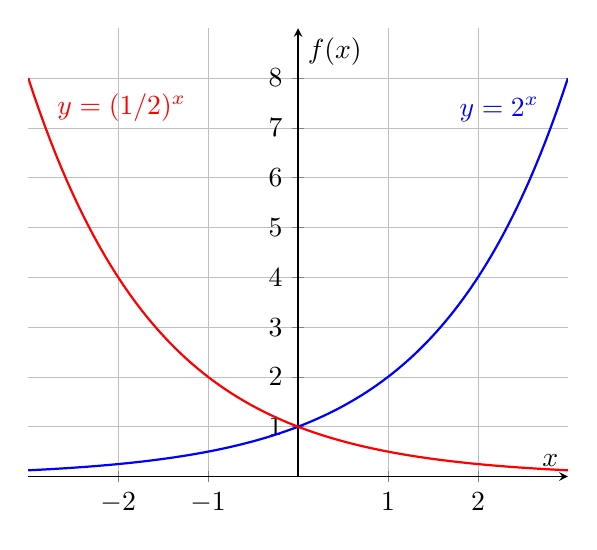
\begin{tikzpicture}
        \begin{axis}[
            axis lines=middle,
            xlabel=$x$,
            ylabel=$f(x)$,
            xmin=-3, xmax=3,
            ymin=0, ymax=9,
            xtick={-2,-1,0,1,2},
            ytick={1,2,3,4,5,6,7,8},
            grid=both,
            grid style={line width=.1pt, draw=gray!10},
            major grid style={line width=.2pt,draw=gray!50},
            domain=-3:3,
            samples=100
        ]
        \addplot[blue, thick] {2^x} node[pos=0.9, above left] {$y=2^x$};
        \addplot[red, thick] {0.5^x} node[pos=0.1, above right] {$y=(1/2)^x$};
        \end{axis}
    \end{tikzpicture}
    \caption{Az $y=2^x$ (növekvő) és $y=(1/2)^x$ (csökkenő) exponenciális függvények grafikonjai.}
    \label{fig:exp_fuggveny}
\end{figure}

\begin{feladatdoboz}[Igaz / Hamis állítások]
Döntsd el, hogy az alábbi állítások igazak vagy hamisak, és indokold válaszodat!
\begin{enumerate}[label=(\alph*)]
    \item Az $f(x) = (0.3)^x$ exponenciális függvény szigorúan monoton növekvő.
    \item Ha $5^x = 5^y$, akkor $x$ szükségképpen egyenlő $y$-nal.
\end{enumerate}
\end{feladatdoboz}

\begin{megoldasdoboz}[Igaz / Hamis állítások]
\begin{enumerate}[label=(\alph*)]
    \item \textbf{Hamis.} Az alap $a = 0.3$. Mivel $0 < 0.3 < 1$, a függvény szigorúan monoton csökkenő.
    \item \textbf{Igaz.} Az exponenciális függvény injektív, azaz kölcsönösen egyértelmű. Ez azt jelenti, hogy minden $y$ értékhez pontosan egy $x$ érték tartozik. Ha két hatvány értéke azonos, és az alap is azonos, akkor a kitevőknek is azonosaknak kell lenniük.
\end{enumerate}
\end{megoldasdoboz}

\section*{Egyszerű exponenciális egyenletek megoldása: Alap azonosítás}

Az exponenciális egyenletek megoldásának egyik leggyakoribb módja, hogy mindkét oldalt azonos alapra hozzuk. Ezt követően az exponenciális függvény injektivitása miatt a kitevőket egyenlővé tehetjük.

\begin{teteldoboz}[Alap azonosítása]
Ha egy exponenciális egyenlet $a^x = a^y$ alakban írható fel ($a>0, a \neq 1$), akkor a megoldása $x = y$.
\end{teteldoboz}

\begin{feladatdoboz}[Egyszerű exponenciális egyenlet]
Oldd meg a következő egyenletet: $2^x = 16$
\end{feladatdoboz}

\begin{megoldasdoboz}[Egyszerű exponenciális egyenlet]
Az egyenlet: $2^x = 16$.
A jobb oldalon lévő 16-ot felírhatjuk 2 hatványaként: $16 = 2^4$.
Így az egyenlet: $2^x = 2^4$.
Mivel az alapok azonosak ($2$), és az exponenciális függvény injektív, a kitevőket egyenlővé tehetjük:
$x = 4$.

\textbf{Ellenőrzés:} $2^4 = 16$, ami helyes.
\textbf{Megoldás:} $x=4$.
\end{megoldasdoboz}

\section*{Bonyolultabb egyenletek alap azonosítással}

Gyakran előfordul, hogy az alapok nincsenek közvetlenül azonos formában, de megfelelő hatványazonosságok segítségével átalakíthatók.

\begin{definiciodoboz}[Fontos hatványazonosságok]
\begin{itemize}
    \item Negatív kitevő: $a^{-n} = \frac{1}{a^n}$
    \item Törtkitevő (gyök): $a^{\frac{m}{n}} = \sqrt[n]{a^m}$
    \item Hatvány hatványa: $(a^m)^n = a^{m \cdot n}$
\end{itemize}
\end{definiciodoboz}

\begin{feladatdoboz}[Exponenciális egyenlet törtkitevővel]
Oldd meg a következő egyenletet: $3^x = \frac{1}{27}$
\end{feladatdoboz}

\begin{megoldasdoboz}[Exponenciális egyenlet törtkitevővel]
Az egyenlet: $3^x = \frac{1}{27}$.
Először a jobb oldalon lévő 27-et írjuk fel 3 hatványaként: $27 = 3^3$.
Így az egyenlet: $3^x = \frac{1}{3^3}$.
A negatív kitevős azonosságot alkalmazva: $\frac{1}{3^3} = 3^{-3}$.
Tehát az egyenlet: $3^x = 3^{-3}$.
Mivel az alapok azonosak, a kitevőket egyenlővé tehetjük:
$x = -3$.

\textbf{Ellenőrzés:} $3^{-3} = \frac{1}{3^3} = \frac{1}{27}$, ami helyes.
\textbf{Megoldás:} $x=-3$.
\end{megoldasdoboz}

\begin{feladatdoboz}[Többlépcsős exponenciális egyenlet]
Oldd meg a következő egyenletet: $4^{x+1} = 8^{2x-1}$.
\begin{enumerate}[label=(\alph*)]
    \item Hozd közös alapra az egyenlet mindkét oldalát! (Tipp: a 2-es alap ideális.)
    \item Egyszerűsítsd a hatványkitevőket!
    \item Oldd meg az így kapott lineáris egyenletet $x$-re!
\end{enumerate}
\end{feladatdoboz}

\begin{megoldasdoboz}[Többlépcsős exponenciális egyenlet]
\begin{enumerate}[label=(\alph*)]
    \item Az egyenlet $4^{x+1} = 8^{2x-1}$.
    A 4 felírható $2^2$-ként, a 8 pedig $2^3$-ként.
    Behelyettesítve: $(2^2)^{x+1} = (2^3)^{2x-1}$.
    \item A hatvány hatványozása szabályt $( (a^m)^n = a^{m \cdot n} )$ alkalmazva:
    $2^{2(x+1)} = 2^{3(2x-1)}$
    $2^{2x+2} = 2^{6x-3}$
    \item Mivel az alapok azonosak, a kitevőknek is azonosaknak kell lenniük:
    $2x+2 = 6x-3$
    Rendezzük az egyenletet:
    $2+3 = 6x-2x$
    $5 = 4x$
    $x = \frac{5}{4}$

\textbf{Ellenőrzés:}
Bal oldal: $4^{\frac{5}{4}+1} = 4^{\frac{9}{4}} = (2^2)^{\frac{9}{4}} = 2^{2 \cdot \frac{9}{4}} = 2^{\frac{9}{2}} = \sqrt{2^9} = \sqrt{512}$.
Jobb oldal: $8^{2 \cdot \frac{5}{4}-1} = 8^{\frac{5}{2}-1} = 8^{\frac{3}{2}} = (2^3)^{\frac{3}{2}} = 2^{3 \cdot \frac{3}{2}} = 2^{\frac{9}{2}} = \sqrt{2^9} = \sqrt{512}$.
A bal és jobb oldal megegyezik, a megoldás helyes.
\textbf{Megoldás:} $x = \frac{5}{4}$.
\end{enumerate}
\end{megoldasdoboz}

\section*{Helyettesítéses módszer (Segédváltozó bevezetése)}

Bizonyos exponenciális egyenletek nem hozhatók közvetlenül azonos alapra. Ilyenkor a segédváltozó bevezetése segíthet, ami az egyenletet egy ismertebb formára, például másodfokú egyenletre alakítja.

\begin{teteldoboz}[Helyettesítéses módszer]
Ha egy exponenciális egyenlet $A \cdot (a^x)^2 + B \cdot a^x + C = 0$ alakú, akkor bevezethetjük a $y = a^x$ segédváltozót. Ekkor az egyenlet $A y^2 + B y + C = 0$ másodfokú egyenletté alakul, amelyet $y$-ra megoldhatunk. Az $y$ értékekből ezután vissza kell számolni az eredeti $x$ ismeretlent. Fontos: $a^x > 0$ minden valós $x$-re, így $y$ is csak pozitív lehet.
\end{teteldoboz}

\begin{feladatdoboz}[Helyettesítéses exponenciális egyenlet]
Oldd meg a következő egyenletet: $9^x - 4 \cdot 3^x + 3 = 0$.
\begin{enumerate}[label=(\alph*)]
    \item Alakítsd át az egyenletet úgy, hogy felismerhető legyen a segédváltozó bevezetésének lehetősége!
    \item Vezess be segédváltozót, és oldd meg a kapott másodfokú egyenletet!
    \item Számold ki az eredeti ismeretlen ($x$) értékét a segédváltozó megoldásaiból!
\end{enumerate}
\end{feladatdoboz}

\begin{megoldasdoboz}[Helyettesítéses exponenciális egyenlet]
\begin{enumerate}[label=(\alph*)]
    \item Az egyenlet: $9^x - 4 \cdot 3^x + 3 = 0$.
    Vegyük észre, hogy $9^x = (3^2)^x = (3^x)^2$.
    Így az egyenlet átírható a következőképpen: $(3^x)^2 - 4 \cdot 3^x + 3 = 0$.
    \item Vezessük be a segédváltozót: $y = 3^x$.
    Ekkor az egyenlet másodfokú egyenletté alakul: $y^2 - 4y + 3 = 0$.
    Ezt az egyenletet megoldhatjuk a másodfokú megoldóképlettel vagy szorzattá alakítással.
    $(y-1)(y-3) = 0$
    A gyökök: $y_1 = 1$ és $y_2 = 3$.
    Mindkét gyök pozitív, tehát alkalmasak az exponenciális függvény értékeként.
    \item Most visszahelyettesítjük az $y = 3^x$ kifejezésbe, hogy meghatározzuk $x$-et:
    \begin{itemize}
        \item Első eset: $y_1 = 1$
        $3^x = 1$
        Mivel $3^0 = 1$, ebből következik, hogy $x_1 = 0$.
        \item Második eset: $y_2 = 3$
        $3^x = 3$
        Mivel $3^1 = 3$, ebből következik, hogy $x_2 = 1$.
    \end{itemize}

\textbf{Ellenőrzés:}
$x_1=0$: $9^0 - 4 \cdot 3^0 + 3 = 1 - 4 \cdot 1 + 3 = 1 - 4 + 3 = 0$. (Helyes)
$x_2=1$: $9^1 - 4 \cdot 3^1 + 3 = 9 - 4 \cdot 3 + 3 = 9 - 12 + 3 = 0$. (Helyes)
\textbf{Megoldások:} $x_1 = 0$ és $x_2 = 1$.
\end{enumerate}
\end{megoldasdoboz}

\end{document}